% !TEX program = xelatex
% RAI Risk Taxonomy Technical Report 2.0, journal-style English edition.
\documentclass[11pt,a4paper]{article}
\usepackage[a4paper,top=22mm,bottom=24mm,left=22mm,right=22mm]{geometry}
\usepackage{fontspec}
\usepackage{microtype}
\usepackage{booktabs,longtable,tabularx,array}
\usepackage{enumitem}
\usepackage{amsmath,amssymb}
\usepackage{graphicx}
\usepackage{float}
\usepackage{pgfplots}
\usepackage{fancyhdr}
\usepackage[title]{appendix}
\usepackage[hidelinks]{hyperref}
\pgfplotsset{compat=1.18}

% Portable font setup: canonical fonts on macOS, TeX Gyre fallbacks elsewhere.
\IfFileExists{/System/Library/Fonts/Menlo.ttc}{%
  \setmainfont{Times New Roman}\setsansfont{Arial}\setmonofont{Menlo}%
  \newfontfamily\krfont{Apple SD Gothic Neo}%
}{%
  \setmainfont{TeX Gyre Termes}\setsansfont{TeX Gyre Heros}\setmonofont{TeX Gyre Cursor}%
  \newfontfamily\krfont{Noto Sans CJK KR}%
}
% Korean text support: wrap Hangul in \ko{...} (fixes missing-glyph breakage).
\newcommand{\ko}[1]{{\krfont #1}}
\setlength{\parindent}{1.4em}
\setlength{\parskip}{0pt}
\setlength{\emergencystretch}{2em}
\newcommand{\code}[1]{\texttt{#1}}
\newcommand{\pct}[1]{#1\%}
\newcolumntype{Y}{>{\raggedright\arraybackslash}X}
\newcolumntype{L}[1]{>{\raggedright\arraybackslash}p{#1}}

\definecolor{natureblue}{HTML}{0072B2}
\definecolor{naturevermillion}{HTML}{D55E00}
\definecolor{naturegreen}{HTML}{009E73}
\definecolor{naturegrey}{HTML}{6B6B6B}
\definecolor{naturelight}{HTML}{D9D9D9}

\pgfplotsset{
  natureaxis/.style={
    axis x line*=bottom,
    axis y line*=left,
    axis line style={black, line width=0.6pt},
    tick align=outside,
    tick style={black, line width=0.5pt},
    tick label style={font=\sffamily\footnotesize, color=black},
    label style={font=\sffamily\small, color=black},
    title style={font=\sffamily\small, color=black},
    legend style={draw=none, fill=none, font=\sffamily\footnotesize},
    grid=none,
    clip=false
  }
}

\pagestyle{fancy}
\setlength{\headheight}{14pt}
\fancyhf{}
\lhead{\footnotesize RAI Risk Taxonomy}
\rhead{\footnotesize Technical Report 2.0}
% Journal-style restructured edition (v2.17.1 state), generated 2026-07-22.
\cfoot{\footnotesize\thepage}
\hypersetup{
  pdftitle={RAI Risk Taxonomy Technical Report 2.0},
  pdfauthor={RAI Risk Taxonomy Project}
}

\title{\vspace{-1.3cm}\bfseries\Large RAI Risk Taxonomy 2.0:\\[3pt]
Top-down evidence selection and staged classification of 1,711 global AI risks}
\author{RAI Risk Taxonomy Project}
\date{21 July 2026}


\begin{document}

\begin{center}
{\LARGE\bfseries RAI Risk Taxonomy 2.0:\\[2pt]
Top-down evidence selection and staged classification of 1{,}711 global AI risks\par}
\vspace{8pt}
{\large RAI Risk Taxonomy Project\par}
\vspace{2pt}
22 July 2026 \,·\, journal edition, release state v2.17.1
\end{center}

\begin{abstract}
\noindent
We present a reproducible, top-down account of the evidence and classification
pipeline behind RAI Risk Taxonomy 2.0. An integrated evidence space of
3{,}906{,}767 AI records (papers, policy reports, patents) is filtered to an
82{,}971-record AI-risk evidence view, from which 1{,}711 canonical L4 risk
cards are constructed, level-validated, and assigned to 50 semantic L3
families under a strict L0--L4 hierarchy; the 182-card Physical AI taxonomy is
preserved as a locked gold set. Classification proceeds through a strict
open-set gate, a suitability-ranked relaxation, and a forced-path completion,
followed by expert review and guarded constrained-EM audits; every algorithmic
or forced placement remains flagged for human adjudication through an explicit
HOLD review state (727 cards, 42.5\%, at v2.17.1). A full-release BGE-M3
validation finds statistically non-random semantic structure (permutation
$p=0.0002$) and shows that the post-audit non-HOLD subset reaches 79.3\%
top-1 and 97.4\% top-5 centroid containment, while global reliability of the
consolidated 50-family partition remains undemonstrated. We specify every
evidence filter, classification rule, and validation limit, and we document
why HOLD concentration reflects cross-cutting risks and category overlap
under a single-parent hierarchy rather than mere misclassification.
\end{abstract}

\noindent\textbf{Keywords:} AI risk taxonomy; evidence synthesis; open-set
classification; semantic mapping; Physical AI; responsible AI.

\section{Introduction}
\label{sec:intro}

A taxonomy can appear complete while concealing uncertainty in its source
corpus, unit of analysis, or placement rules. RAI Risk Taxonomy 2.0 therefore
separates four quantities that must not be conflated: the size of the integrated
AI evidence space, the size of the AI-risk evidence view, the number of
canonical L4 risk cards, and the number of L4 cards assigned to L3. The central
result is a top-down evidence-to-taxonomy chain of 3,906,767 records, 82,971
AI-risk records, 1,726 candidate L4 rows, 1,725 exact-deduplicated candidates,
1,711 level-validated L4 cards, and 1,711 L3-assigned cards.

The transitions do not all preserve the same statistical unit. The first two
stages count documents or patent records. The third and fourth stages count
canonical risk concepts. Consequently, the 82,971 evidence records are not a
one-to-one parent table from which every L4 card was mechanically generated.
They form an auditable evidence view supporting corpus coverage and risk
interpretation, whereas the L4 registry integrates risk taxonomies, benchmarks,
standards, and linked evidence through a source crosswalk.


The remainder of this paper is organized as an academic report. Section~\ref{sec:data}
describes the top-down construction of the evidence corpus and the canonical L4
registry. Section~\ref{sec:methods} specifies the classification methodology,
including the staged hierarchy-blind procedure, the guarded constrained-EM audit,
and the HOLD review policy. Section~\ref{sec:results} reports release composition
and reliability validation for the current release state (v2.17.1).
Section~\ref{sec:discussion} interprets the validation evidence and its limits, and
Section~\ref{sec:conclusion} states the release decision and review priorities.
Version-by-version engineering history, detailed review policies, exploratory
analyses, and reporting conventions are collected in the appendices.

\section{Evidence corpus and canonical L4 registry}
\label{sec:data}

\subsection{Integrated AI evidence space}

The top-level dataset contains 3,906,767 records from three source families:
1,749,159 papers, 125,372 policy reports, and 2,032,236 patents. Paper records
originate from the local global Web of Science AI collections. Policy records
combine the reviewed curated AI-policy master with the broader policy-materials
collection. Patent records originate from the stage-2 AI patent master.

Records are standardized to a common schema and retained only when a non-empty
title is available. Deduplication is performed within document type and
analytical category. The ordered key hierarchy is patent application ID for
patents, followed by DOI, source record ID, URL, and a normalized
title-year-institution fallback. Cross-category overlap is intentionally
retained because AI, AI infrastructure, Physical AI, and AI risk are analytical
views rather than mutually exclusive partitions.

\subsection{Integrated AI-risk evidence view}

The AI-risk evidence view contains 82,971 records: 50,375 papers, 938 policy
reports, and 31,658 patents. Its inclusion rule is source-governed rather than a
single keyword query. Papers combine curated academic risk references, the
clean and integrated AI-risk paper corpora, Physical AI safety benchmarks, and
verified paper records from the top-200 evidence set. Policy reports combine
curated risk-policy references with verified report records. Patents combine
curated risk-patent references with verified patent records. Record-type filters
are applied before the same title-validity and within-category deduplication
rules used at Stage A.

This view represents 2.1\% of the integrated AI evidence space. Because the
source collections and analytical categories can overlap, this percentage is a
descriptive ratio, not the estimated prevalence of risk research in all AI
scholarship.

\subsection{Canonical L4 registry}

The unit changes from evidence record to risk concept. Source risk IDs are
joined through the source crosswalk, semantically redundant cards are reviewed,
and one canonical row is retained per L4 failure mode or harm mechanism.
Permanent identifiers \code{RAI4-0001} through \code{RAI4-1726} are allocated
independently of the risk label. The initial result is 1,726 candidate L4 rows. Automatic
deduplication is restricted to pairs whose normalized label and mechanism-only
definition are both exactly equal; semantic-similarity thresholds are not used.
This merges \code{RAI4-1606} into \code{RAI4-1083}, retains both source references,
and yields 1,725 exact-deduplicated candidates. The retired ID remains in the
crosswalk. The registry includes the 182-card Physical AI taxonomy as a
protected mapping set.

The ratio of L4 cards to AI-risk evidence records is 2.1\%. It is reported only
as a scale-change diagnostic: one document may support multiple risks, and one
risk may be supported by multiple documents. It is not a document acceptance
rate.

\subsection{Taxonomy-level validation}

The deployed Physical AI site is the authoritative source for its 24 L3 names
and 182 L4 cards. Its live HTML was byte-identical to the local repository
snapshot used for this check. We compare the English component of each
authoritative Physical L3 name with every candidate L4 label after NFKC
normalization, case folding, ampersand normalization, and removal of
non-alphanumeric separators. A card is excluded only when these normalized
labels are exactly equal; semantic similarity and definition similarity are not
used. Fourteen L4 rows match category names and are retired as taxonomy-level
leakage, including \code{RAI4-0553} ``Accidental harm'', which maps to Physical
L3 \code{P3.1}. Their definitions and references remain in the audit crosswalk.
This yields 1,711 canonical L4 cards without changing any of the protected 182
Physical L4 mappings.

\subsection{Assignment coverage overview}

The operational policy assigns all 1,711 canonical L4 cards to an L3 node
(100.0\%). The original three-stage classifier used 50 L3 nodes and retained
76 decision-review markers after level validation. Release v2.7.0 then removed
1,129 instances of circular taxonomy prose from non-Physical definitions,
performed evidence-constrained mapping review, and marked 692 cards where the
available definition and evidence did not justify an approved taxonomic fit.
The v2.8.0 Agentic expansion evaluates every non-Physical card while locking
all 182 Physical mappings. It moves 31 cards into four new L3 nodes and clears
seven review markers, leaving 685 cards (40.0\%) marked \code{HOLD}. Releases
v2.9.0 to v2.12.0 then audit Anthropomorphism, Goal Misalignment, and Copyrights,
leaving 689 cards (40.3\%) marked \code{HOLD}. Release v2.13.0 differentiates
three overlapping Memory cards and places all three under source-entailment or
near-duplicate scope review, yielding 692 held cards (40.4\%). Release v2.14.0
then retires the four sparse Agentic families and force-migrates all 39 affected
cards; 28 newly enter review, yielding 720 held cards (42.1\%). The marker
is internal review metadata on an already assigned card, not a separate L1,
L2, or L3 category.

\begin{figure}[H]
\centering
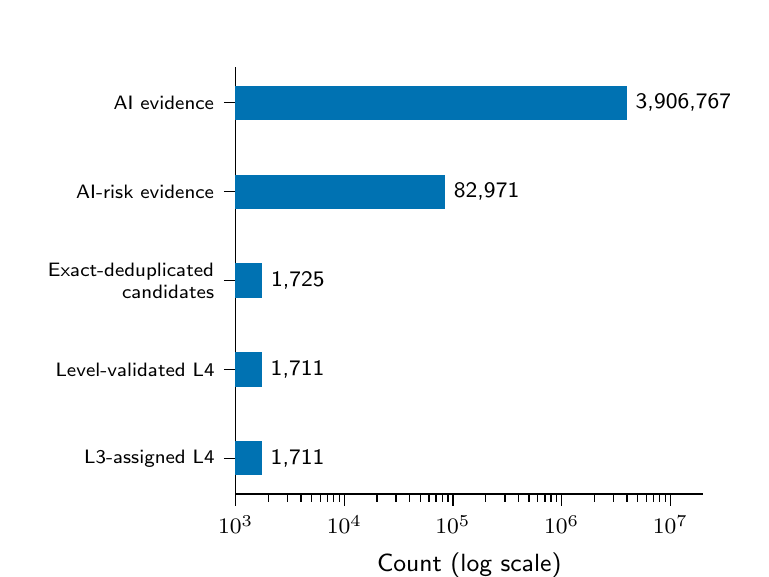
\begin{tikzpicture}
\begin{axis}[
  natureaxis,
  xbar,
  xmode=log,
  log origin=infty,
  log basis x=10,
  xmin=1000,
  xmax=20000000,
  width=0.62\linewidth,
  height=7.0cm,
  xlabel={Count (log scale)},
  symbolic y coords={L3-assigned L4,Level-validated L4,Exact-deduplicated candidates,AI-risk evidence,AI evidence},
  ytick={L3-assigned L4,Level-validated L4,Exact-deduplicated candidates,AI-risk evidence,AI evidence},
  yticklabels={L3-assigned L4,Level-validated L4,Exact-deduplicated candidates,AI-risk evidence,AI evidence},
  yticklabel style={font=\sffamily\scriptsize,text width=2.25cm,align=right},
  bar width=12pt,
  point meta=explicit symbolic,
  nodes near coords={\pgfplotspointmeta},
  nodes near coords style={font=\sffamily\footnotesize, anchor=west},
]
\addplot[fill=natureblue, draw=natureblue] coordinates {
  (1711,L3-assigned L4) [1,711]
  (1711,Level-validated L4) [1,711]
  (1725,Exact-deduplicated candidates) [1,725]
  (82971,AI-risk evidence) [82,971]
  (3906767,AI evidence) [3,906,767]
};
\end{axis}
\end{tikzpicture}
\caption{\textbf{Top-down evidence and taxonomy funnel.} Counts move from
document/patent records to canonical risk concepts at the transition from
AI-risk evidence to L4. The logarithmic axis preserves visibility across four
orders of magnitude.}
\label{fig:funnel}
\end{figure}

\begin{table}[H]
\centering
\caption{Top-down stages, counts, and inclusion filters.}
\label{tab:funnel}
\small
\begin{tabularx}{\linewidth}{L{0.18\linewidth}r L{0.20\linewidth}Y}
\toprule
Stage & Count & Unit & Principal filter \\
\midrule
AI evidence & 3,906,767 & Document or patent record & AI source collections; valid title; standardized schema; within-type/category deduplication. \\
AI-risk evidence & 82,971 & Document or patent record & Curated/integrated risk sources; record-type inclusion; valid title; within-type/category deduplication. \\
Exact-deduplicated candidates & 1,725 & Risk card & Exact normalized label and core-definition match only; one retired ID mapped to its canonical card. \\
Canonical L4 & 1,711 & Risk card & Exact normalized-label exclusion against 24 authoritative Physical L3 names; 14 level leaks retired; all 182 Physical L4 cards preserved. \\
L3 assigned & 1,711 & Risk card & Protected Physical mapping or staged non-Physical placement; 689 decision-required cards remain assigned and marked \code{HOLD}. \\
\bottomrule
\end{tabularx}
\end{table}

\section{Classification methodology}
\label{sec:methods}

\subsection{Hierarchy and protected Physical AI mapping}

The taxonomy uses three canonical L2 categories (Interaction Safety, System
Safety, Societal Safety) plus a HOLD review overlay, and permanent
\code{RAI4-\#\#\#\#} identifiers that are independent of taxonomy placement
(Appendix~\ref{app:history}).

The 182 L4-to-L3 mappings inherited from the Physical AI taxonomy are treated
as the locked gold set. Later stages cannot change these paths. Before the
taxonomy-level exclusion, the remaining 1,543 candidates enter the
hierarchy-blind classification procedure. Legacy global
L0-L3 labels, source families, and source-ID prefixes remain reference metadata
and are excluded from prediction features.

\subsection{Stage 1: strict open-set gate}

The input for each non-Physical card is the L4 label, a mechanism-only
definition with hierarchy restatements removed, and the evidence title. Let
$s_{sem}$ be the top-1 semantic score, $s_{comp}$ the top-1 composite score,
$m_{sem}$ and $m_{comp}$ their respective top-1 margins, and $v_{anchor}$ the
number of anchor views selecting the same L3. A candidate is retained only when
all seven conditions hold:

\begin{enumerate}[leftmargin=2em]
  \item exactly one L3 is rule-eligible;
  \item the rule winner, semantic top-1, and composite top-1 are identical;
  \item $s_{sem}\geq0.55$ and $s_{comp}\geq0.54$;
  \item $m_{sem}\geq0.035$ and $m_{comp}\geq0.035$;
  \item $v_{anchor}\geq2$ across three anchor views;
  \item no gap sentinel, multi-mechanism flag, or Physical-boundary flag is present; and
  \item two independent expert agents approve the same exact L3.
\end{enumerate}

This gate yields 37 new expert-consensus proposals. Together with the 182
Physical locks, Stage 1 assigns 219 cards and withholds 1,507.

\subsection{Stage 2: suitability-ranked relaxation}

Stage 2 preserves all 219 protected assignments and computes
\begin{equation}
S_2=0.55q_{sem}+0.20q_{sm}+0.10q_{cm}+0.10q_{vote}+0.05q_{rule}-p_{gap},
\end{equation}
where
\begin{align}
q_{sem}&=\operatorname{clip}\left(\frac{s_{sem}-0.45}{0.25},0,1\right),\\
q_{sm}&=\operatorname{clip}\left(\frac{m_{sem}}{0.05},0,1\right),\\
q_{cm}&=\operatorname{clip}\left(\frac{m_{comp}}{0.05},0,1\right),\\
q_{vote}&=v_{anchor}/3,\\
q_{rule}&=\mathbf{1}[\text{at least one eligible L3}],\\
p_{gap}&=0.05\,\mathbf{1}[\text{gap sentinel present}].
\end{align}

$S_2$ is a deterministic ranking score rather than a calibrated probability.
Stage 2 first preserves 55 hard holds. It then orders the remaining holds by
ascending $S_2$, with permanent RAI4 ID as the tie breaker, and reserves the
lowest 118. Thus $55+118=173$ cards remain unresolved and 1,553 cards are
assigned (90.0\%).

\subsection{Stage 3: forced-path completion}

Stage 3 preserves the 1,553 Stage 2 paths and assigns only the 173 unresolved
cards to the hierarchy-blind top-1 L3 already stored in the score artifact.
This produces 1,726 operational paths but does not validate taxonomy fit. Each
new path retains its original hold reason, score, review priority, and
\code{human\_approved=false} marker.

The final policy marks five difficult-case families for decision review:
23 Physical-scope reviews, 17 expert rejections, 7 expert disagreements,
6 multi-mechanism cases, and 2 low-absolute-fit cases. Their forced L3 path
remains populated and \code{decision\_required=true}. The
remaining 118 quota holds also retain their forced paths and review metadata.

\subsection{Constrained-EM audit procedure}
\label{sec:cem}

Later audits do not apply unconstrained nearest-centroid output. Each audit
allows only the selected source L3 cards to move, treats all other cards as
fixed anchors, excludes every Physical destination, and recomputes candidate
centroids until no assignment changes. The composite score is
\begin{equation}
S(i,k)=0.60\,c(i,k)+0.30\,d(i,k)+0.10\,w(i,k),
\end{equation}
where $c$ is current-centroid cosine similarity, $d$ is L3-definition cosine
similarity, and $w$ is TF-IDF keyword cosine similarity. A destination must
improve on the source by at least 0.020 and have keyword cosine of at least
0.015. Agentic destinations additionally require an explicit autonomous
execution mechanism, and destination-specific definition guards reject
matches caused by generic shared terms.

The cumulative audits move three Anthropomorphism cards in v2.9.0, five Goal
Misalignment cards in v2.10.0, four Copyrights cards in v2.11.0, and eight
additional Anthropomorphism cards in v2.12.0. Every such move remains
\code{HOLD} until human adjudication. The final domain counts are 1,165 General,
364 Agentic, and 182 Physical cards; the review queue contains 689 cards.

\subsection{Definition revision and guarded audit (v2.17.0)}

Release v2.17.0 applies an expert editorial pass to the non-Physical registry
while keeping all 182 Physical cards byte-identical. The pass rewrites 147
title and definition mismatch candidates identified by the v2.16.0 remediation
audit into mechanism-only bilingual definitions, renames 15 non-descriptive
labels with the original label preserved in provenance, applies 187 mechanical
hygiene fixes (hyphenation artifacts, missing final punctuation, duplicated
tokens) to the remaining non-Physical definitions, and attaches five
externally verified governance references (NIST AI 100-1; OWASP Top 10 for LLM
Applications 2025) to directly matching cards. Every textual change carries
\code{human\_review\_status=pending} and retains the original text in a
\code{definition\_revision} record; no HOLD marker is cleared by this pass.

The revised card text is then re-audited with the constrained-EM procedure of Section~\ref{sec:cem} using the pinned local BGE-M3 snapshot
\code{5617a9f61b028005a4858fdac845db406aefb181}. The unguarded BGE-M3 control
run produced 151 candidate moves and converged after six non-zero update
passes, followed by a seventh zero-move pass. This result is intentionally
used as sensitivity evidence rather than as automatic ground truth: it shows
that the edited definitions expose many plausible local alternatives, but the
volume of candidates is too high for direct publication without human review.
The published v2.17.0 placement layer therefore preserves the guarded RC
policy: 22 defensible proposals are recorded, of which 14 produce actual
\code{primary\_l3\_id} changes and 8 update the semantic path of cards that
were already in a HOLD review path. All 22 movers carry
\code{decision\_required=true}; the review queue grows from 720 to 734. No
Physical path changed.

The apparent difference between 22 proposals and 14 primary moves is therefore
structural, not an accounting error. A non-HOLD card stores its operational L3
in \code{primary\_l3\_id}, so a guarded proposal changes that field. A card
that is already in a HOLD path keeps \code{primary\_l3\_id} at the HOLD node
and stores the proposed semantic family in \code{hold\_semantic\_path}. Those
eight cards are valid reassignment proposals but do not appear as primary L3
moves in a direct card-to-card diff.

\subsection{HOLD review policy}
\label{sec:hold}

\code{HOLD} is the public rendering of \code{decision\_required=true}. In
v2.15.0 it is a review-path L2 under General and Agentic AI, not a semantic risk
family. A held card has one navigable HOLD path and retains its prior semantic
L3 candidate as explicit lineage metadata; neither path is human-approved
ground truth. The state is set by a hard qualitative
trigger or by a pending algorithmic-review trigger. It is cleared only by a
recorded human decision that reconciles the label, mechanism-only definition,
evidence, and destination definition; absence of a competing score alone is
not sufficient.

\paragraph{Quantitative criteria.}
Quantitative measurements control automatic eligibility and review priority,
not semantic truth. The following rules are applied or reported:
\begin{enumerate}[leftmargin=2em]
  \item Stage 1 automatic acceptance requires $s_{sem}\geq0.55$,
  $s_{comp}\geq0.54$, both margins at least 0.035, at least two of three anchor
  votes, exact agreement of the rule, semantic, and composite winners, and two
  matching expert-agent approvals. Failure prevents automatic clearance.
  \item Stage 2 uses the deterministic suitability score $S_2$ defined above;
  the lowest-ranked reserve and every hard hold retain decision metadata after
  forced operational assignment.
  \item A constrained-EM move requires composite improvement of at least 0.020
  over the source and keyword cosine of at least 0.015. Passing these thresholds
  permits a proposal but never clears \code{HOLD} automatically.
  \item For v2.12.0 audit prioritization, a top-two cosine margin below 0.020 is
  high priority, a margin from 0.020 to below 0.050 is medium priority, and a
  margin of at least 0.050 is lower priority. Released-L3 rank outside the top
  three or per-card agreement below 80.0\% under $\sigma=0.05$ perturbation is
  an additional instability signal.
  \item Strong geometric support is reported only when top-1 containment is at
  least 90.0\%, top-2 containment at least 95.0\%, the matched-size permutation
  test has $p<0.001$, and perturbation agreement remains at least 97.0\% through
  $\sigma=0.05$. These are validation thresholds, not substitutes for the
  qualitative tests below.
\end{enumerate}

The qualitative retention criteria are listed in Appendix~\ref{app:holdpolicy}.

\section{Results}
\label{sec:results}

\subsection{Evidence composition}

Papers account for 44.8\% of the integrated AI evidence space, policy reports
for 3.2\%, and patents for 52.0\%. Within the AI-risk evidence view, the
corresponding shares are 60.7\%, 1.1\%, and 38.2\%. These shares use one decimal
because their integer component is at least one.

\begin{figure}[H]
\centering
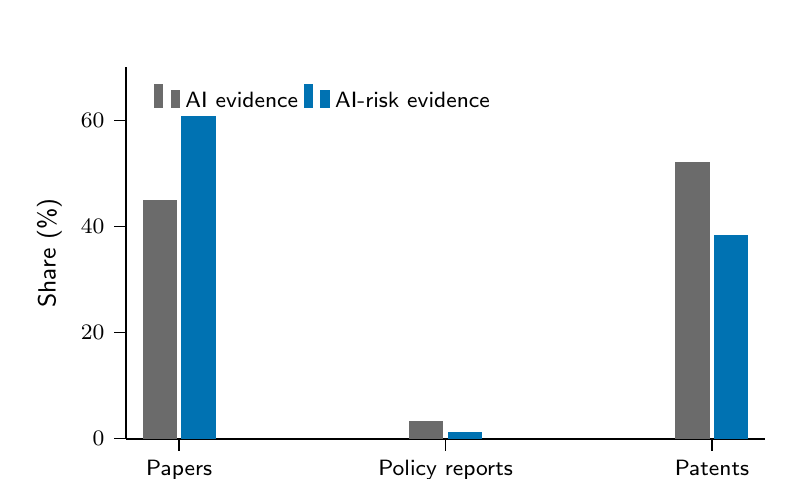
\begin{tikzpicture}
\begin{axis}[
  natureaxis,
  ybar,
  ymin=0,
  ymax=70,
  width=0.80\linewidth,
  height=6.3cm,
  ylabel={Share (\%)},
  symbolic x coords={Papers,Policy reports,Patents},
  xtick=data,
  bar width=12pt,
  legend columns=2,
  legend pos=north west,
]
\addplot[fill=naturegrey, draw=naturegrey] coordinates {(Papers,44.8) (Policy reports,3.2) (Patents,52.0)};
\addplot[fill=natureblue, draw=natureblue] coordinates {(Papers,60.7) (Policy reports,1.1) (Patents,38.2)};
\legend{AI evidence,AI-risk evidence}
\end{axis}
\end{tikzpicture}
\caption{\textbf{Source-family composition.} Percentages compare document-type
composition within the integrated AI evidence space and the AI-risk evidence
view.}
\label{fig:composition}
\end{figure}

\subsection{Hierarchy coverage}

The final policy assigns all 1,711 canonical cards (100.0\%); 720 assigned
cards (42.1\%) carry the \code{HOLD} marker. Of all cards, 1,193 are General,
336 are Agentic AI, and 182 are Physical AI. Their shares are 69.7\%, 19.6\%,
and 10.6\%, respectively. All 50 semantic L3 nodes contain at least one
non-HOLD card. The two HOLD review-path L3 nodes contain 626 General and 94
Agentic cards, respectively.
Anthropomorphism is the largest L3 with 234 cards (13.7\%); the five largest
L3 nodes jointly contain 41.6\%.

\begin{figure}[H]
\centering
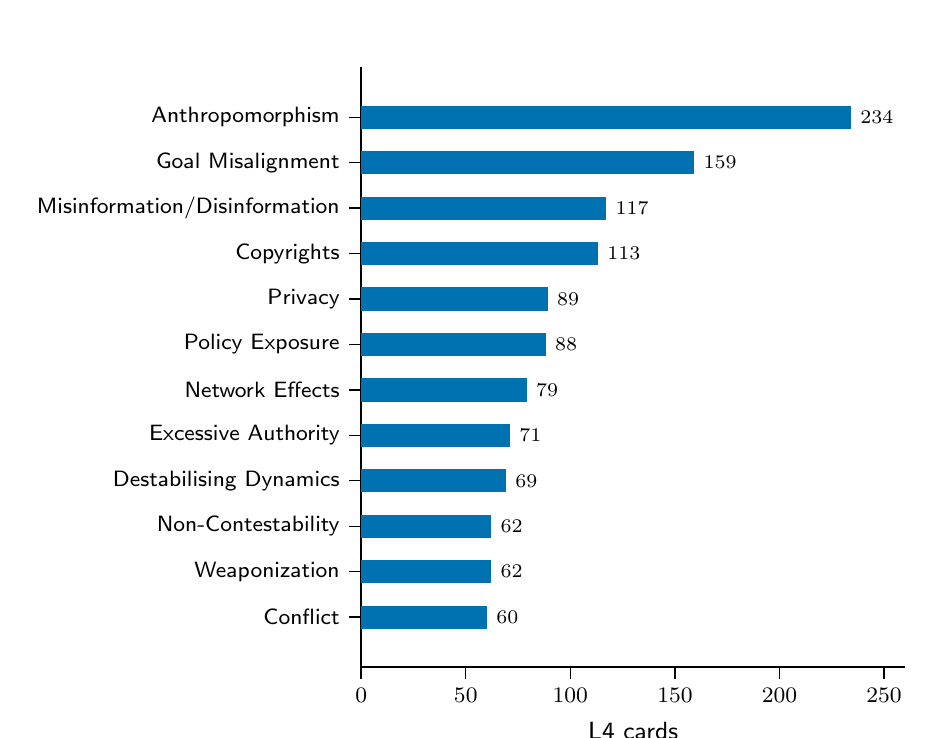
\begin{tikzpicture}
\begin{axis}[
  natureaxis,
  xbar,
  xmin=0,
  xmax=260,
  width=0.70\linewidth,
  height=9.2cm,
  xlabel={L4 cards},
  symbolic y coords={Conflict,Weaponization,Non-Contestability,Destabilising Dynamics,Excessive Authority,Network Effects,Policy Exposure,Privacy,Copyrights,Misinformation/Disinformation,Goal Misalignment,Anthropomorphism},
  ytick=data,
  bar width=8pt,
  nodes near coords,
  nodes near coords style={font=\sffamily\scriptsize, anchor=west},
]
\addplot[fill=natureblue, draw=natureblue] coordinates {
 (60,Conflict) (62,Weaponization) (62,Non-Contestability)
 (69,Destabilising Dynamics) (71,Excessive Authority) (79,Network Effects)
 (88,Policy Exposure) (89,Privacy) (113,Copyrights)
 (117,Misinformation/Disinformation) (159,Goal Misalignment) (234,Anthropomorphism)
};
\end{axis}
\end{tikzpicture}
\caption{\textbf{Largest L3 nodes in the final policy view.} The figure shows
the eleven largest L3 nodes. Counts include assigned cards marked
\code{HOLD}.}
\label{fig:l3}
\end{figure}

After the v2.17.0 guarded audit and the minimal v2.17.1 Physical transfer
(Appendix~\ref{app:history}), the public release state comprises 189
Physical-path cards and 727 HOLD cards (42.5\%); the locked 182-card Physical
source set is unchanged.

\subsection{HOLD composition at v2.17.0}

The v2.17.0 HOLD queue contains 734 cards, or 42.9\% of the 1,711-card
release. HOLD is not a semantic failure label; it is an operational review
state assigned when the evidence, L4 mechanism, and candidate L3 definition do
not jointly justify automatic release as a human-approved mapping. To make the
review queue actionable, the release groups HOLD reasons into mutually
exclusive operational causes using \code{decision\_reason},
\code{stage2\_hold\_reason}, and the v2.17.0 guarded remap metadata. The
machine-readable output is stored in
\code{reports/validation/v2.17.0/hold\_reason\_groups/}.

\begin{table}[ht]
\centering
\caption{Primary operational causes of HOLD status in v2.17.0.}
\label{tab:hold-reason-groups-v217}
\begin{tabular}{lrrr}
\toprule
HOLD cause & Cards & Share of HOLD & Share of all L4 \\
\midrule
Taxonomy gap or missing L3 scope & 280 & 38.1\% & 16.4\% \\
Anthropomorphism mechanism ambiguity & 173 & 23.6\% & 10.1\% \\
Overloaded L3 or weak evidence fit & 138 & 18.8\% & 8.1\% \\
Expert disagreement or rejection & 51 & 6.9\% & 3.0\% \\
Retired sparse Agentic L3 migration & 39 & 5.3\% & 2.3\% \\
Guarded BGE-M3 remap review & 26 & 3.5\% & 1.5\% \\
Physical AI lock-scope conflict & 16 & 2.2\% & 0.9\% \\
Low-fit or multi-mechanism residual & 8 & 1.1\% & 0.5\% \\
Other residual review & 3 & 0.4\% & 0.2\% \\
\bottomrule
\end{tabular}
\end{table}

The distribution shows that HOLD is dominated by three causes. First, 280
cards expose a taxonomy gap or missing L3 scope. These cards are not simply
bad assignments; many point to governance, transparency, security,
dependency, environmental, labor, and deliberate-disinformation themes that
are only partially covered by the current 50 semantic L3 families. Second, 173
cards remain held because an Anthropomorphism assignment is not established as
a direct harm mechanism. These cards frequently mention trust, identity,
affective influence, or social interaction, but the definition does not prove
that anthropomorphic design is the operative risk mechanism. Third, 138 cards
sit in overloaded L3 families or have weak evidence fit. Their current L3 may
be operationally usable, but the source evidence is too broad or the L4
mechanism too diffuse for direct release.

\begin{table}[ht]
\centering
\caption{Taxonomy-gap mentions inside the HOLD queue. Multi-tag cards are
counted once per tag.}
\label{tab:hold-taxonomy-gap-v217}
\begin{tabular}{lrr}
\toprule
Taxonomy-gap theme & Mentions & Share of gap mentions \\
\midrule
Governance, audit, and regulation & 87 & 28.8\% \\
Transparency and explainability & 44 & 14.6\% \\
Robustness, alignment, and control & 34 & 11.3\% \\
General AI security & 31 & 10.3\% \\
Dependency and manipulation & 30 & 9.9\% \\
Pluralistic values and stakeholders & 21 & 7.0\% \\
Environment, energy, and resources & 20 & 6.6\% \\
Labor, inequality, and power & 17 & 5.6\% \\
Deliberate disinformation & 16 & 5.3\% \\
Other taxonomy-gap tags & 2 & 0.7\% \\
\bottomrule
\end{tabular}
\end{table}

A HOLD-only BGE-M3 remap probe was also run for the 734 held cards. It found
496 cards whose top-1 semantic L3 differs from the stored HOLD semantic path,
but all 496 are weak-tier candidates under the conservative threshold: no card
met the joint score, margin, and keyword-support requirements for automatic
movement. This confirms that HOLD should be used to prioritize human review,
not to trigger bulk remapping. The highest-priority review queue should start
with taxonomy-gap cards, then Anthropomorphism ambiguity, then overloaded-L3
or weak-evidence cases.

\subsection{Reliability validation}

Reliability is re-evaluated on all 1,711 v2.14.0 paths using dense,
1,024-dimensional BGE-M3 embeddings, seed 20260721, maximum sequence length
256, batch size 32, and L2 normalization. Card text concatenates bilingual L4
labels and definitions; L3 seed text concatenates bilingual L3 labels and
definitions. The procedure reproduces four checks from the prior Technical
Report. This rerun encodes the current v2.14.0 card text and all 50 active L3
seed definitions. It therefore incorporates both the v2.13.0 Memory wording
revisions and the v2.14.0 forced migrations.

First, seed-initialized spherical EM alternates nearest-centroid assignment and
normalized centroid recomputation:
\begin{equation}
z_i^{(t+1)}=\arg\max_k y_i^\top\mu_k^{(t)},\qquad
\mu_k^{(t+1)}=\frac{\sum_{i:z_i=k}y_i}
{\left\|\sum_{i:z_i=k}y_i\right\|_2}.
\end{equation}
Second, top-$k$ containment is the proportion of cards whose published L3 is
among the $k$ nearest centroids calculated from the published partition. Third,
the observed mean within-family cosine is compared with 5,000 label
permutations that exactly preserve family sizes; the p-value uses the plus-one
correction. Fourth, isotropic Gaussian embedding perturbation is repeated 200
times per $\sigma$, and agreement compares perturbed with unperturbed
nearest-centroid assignments.

\begin{figure}[H]
\centering

\includegraphics[width=\textwidth]{../validation/v2.14.0/reliability/reliability_validation.pdf}
\caption{\textbf{Convergence and stability before HOLD separation (v2.14.0).}
All 1,711 cards are assessed while the 720 HOLD cards remain embedded in their
semantic L3 candidates.
(a) Seed-initialized spherical EM reaches a fixed point after 15 iterations.
(b) v2.14.0 top-$k$ containment is compared with the v2.12.0 54-family baseline.
(c) Perturbation stability remains materially similar after consolidation.}
\label{fig:reliability}
\end{figure}

\begin{table}[H]
\centering
\caption{Full-release reliability results before and after L3 consolidation.}
\small
\begin{tabular}{lrr}
\toprule
Metric & v2.12.0 & v2.14.0 \\
\midrule
L3 families & 54 & 50 \\
Cards assessed & 1,711 & 1,711 \\
Mean within-family cosine & 0.770 & 0.768 \\
Median assignment margin & 0.012 & 0.012 \\
Top-1 containment & 64.6\% & 64.7\% \\
Top-2 containment & 78.7\% & 78.6\% \\
Top-3 containment & 86.1\% & 86.1\% \\
Top-5 containment & 93.3\% & 93.1\% \\
Permutation p-value & 0.0002 & 0.0002 \\
Agreement at $\sigma=0.01$ & 94.4\% & 94.5\% \\
Agreement at $\sigma=0.05$ & 72.8\% & 72.8\% \\
\bottomrule
\end{tabular}
\end{table}

The EM objective increases monotonically from 0.661 to 0.800 and reaches zero
reassignments after 15 iterations. The converged unsupervised partition,
however, agrees with only 21.8\% of published paths (adjusted Rand index 0.120;
normalized mutual information 0.402) and proposes 1,338 changes. Numerical
convergence is therefore not evidence that the published semantics are correct.
Published cohesion is 0.7684, above the matched-size null mean of 0.7382 with zero
exceedances in 5,000 permutations (plus-one $p=0.0002$). The taxonomy contains
non-random semantic structure, but its global partition is not robust under the
tested geometry.

\subsection{Reliability at the current release state}

The final sensitivity analysis uses the canonical BGE-M3 encoder, seed
20260721, the same 50 semantic L3 families, 5,000 matched-size permutations,
and the same perturbation grid used in the historical analyses (Appendix~\ref{app:hist}). Table~\ref{tab:v217-bge}
reports the geometry before and after the BGE-M3 constrained audit. HOLD is
reported both included and excluded because the HOLD marker is a review state,
not a semantic L3 family.

\begin{table}[ht]
\centering
\caption{BGE-M3 reliability before and after the v2.17.0 constrained-EM audit.}
\label{tab:v217-bge}
\begin{tabular}{lrrrr}
\toprule
Metric & All, pre & All, post & Non-HOLD, pre & Non-HOLD, post \\
\midrule
Cards assessed & 1,711 & 1,711 & 977 & 977 \\
Top-1 containment & 64.9\% & 69.5\% & 76.8\% & 79.3\% \\
Top-2 containment & 78.9\% & 83.5\% & 88.3\% & 91.6\% \\
Top-3 containment & 85.9\% & 90.4\% & 92.2\% & 94.6\% \\
Top-5 containment & 93.0\% & 95.0\% & 95.6\% & 97.4\% \\
Median assignment margin & 0.0125 & 0.0146 & 0.0240 & 0.0279 \\
Negative-margin share & 35.1\% & 30.5\% & 23.2\% & 20.7\% \\
Permutation $p$ & 0.0002 & 0.0002 & 0.0002 & 0.0002 \\
EM convergence iterations & 25 & 25 & 12 & 12 \\
EM objective at convergence & 0.801 & 0.801 & 0.802 & 0.802 \\
EM agreement with released paths & 20.6\% & 22.3\% & 30.0\% & 31.7\% \\
Agreement at $\sigma=0.01$ & 94.1\% & 94.7\% & 95.6\% & 96.0\% \\
Agreement at $\sigma=0.05$ & 72.3\% & 74.0\% & 78.4\% & 80.0\% \\
\bottomrule
\end{tabular}
\end{table}

Three findings follow. First, the released taxonomy is statistically
non-random under BGE-M3: within-family cohesion exceeds every matched-size
permutation in all four conditions ($p=0.0002$). Second, excluding HOLD
improves every reliability indicator. After the v2.17.0 audit, top-1
containment rises from 69.5\% to 79.3\%, top-5 containment from 95.0\% to
97.4\%, the negative-margin share falls from 30.5\% to 20.7\%, and
$\sigma=0.05$ perturbation stability rises from 74.0\% to 80.0\%. Third, the
constrained audit improves local geometry but does not convert the taxonomy
into a fully validated ground truth. EM-to-release agreement remains modest
(22.3\% with HOLD included; 31.7\% with HOLD excluded), which is expected
because unconstrained spherical EM has no hierarchy, protected Physical lock,
HOLD review state, or policy constraint. The release conclusion therefore
remains \textbf{SHARE WITH CAVEATS}: v2.17.0 is suitable for public review and
navigation, while the 734 HOLD cards and the 22 guarded reassignment proposals
remain priority items for human adjudication.

\subsection{Policy-subset separation}

The current HOLD queue is measurably weaker than the non-HOLD subset under the
same released-centroid geometry. This supports the review marker as a triage
instrument, although it does not prove that every individual marker is correct.

\begin{table}[H]
\centering
\caption{v2.14.0 reliability by policy subset.}
\small
\begin{tabular}{lrrrrr}
\toprule
Subset & Cards & Mean cosine & Median margin & Top-1 & Top-3 \\
\midrule
Physical locked & 182 & 0.817 & 0.038 & 89.0\% & 97.3\% \\
Non-Physical & 1,529 & 0.763 & 0.009 & 61.8\% & 84.8\% \\
HOLD & 720 & 0.759 & 0.004 & 56.1\% & 82.6\% \\
Non-HOLD & 991 & 0.775 & 0.018 & 70.9\% & 88.6\% \\
Forced migrations & 39 & 0.746 & -0.005 & 46.2\% & 71.8\% \\
\bottomrule
\end{tabular}
\end{table}

The HOLD top-1 rate is 14.8 percentage points below the non-HOLD rate, and its
median margin is less than one quarter of the non-HOLD margin. Negative margins
occur for 43.9\% of HOLD cards versus 29.1\% of non-HOLD cards. The protected
Physical subset is substantially stronger, with 89.0\% top-1 and 96.7\% top-2
containment, but remains locked because authority comes from the Physical AI
taxonomy rather than from this geometric diagnostic.

Relative to v2.12.0, v2.14.0 raises global top-1 containment by 0.1 percentage
points, while cohesion decreases by 0.0018, top-2 decreases by 0.1 points, and
$\sigma=0.05$ agreement is unchanged at the displayed precision. These
differences are negligible at global scale. The correct conclusion is therefore
\textbf{SHARE WITH CAVEATS}: the taxonomy has statistically non-random semantic
structure and a useful HOLD separation, but strong global assignment
reliability is not demonstrated.

\section{Discussion}
\label{sec:discussion}

\subsection{What the validation does and does not establish}

\textbf{Sparse-family consolidation: OPERATIONAL PASS WITH REVIEW.} Exactly 39
cards were migrated, no Physical path or L4 identity changed, all four retired
families were archived, and every migrated card remains \code{HOLD}. The weak
migrated-subset geometry prohibits interpreting the destinations as approved
ground truth.

\textbf{Full 50-family taxonomy: NOT YET DEMONSTRATED.} The permutation test
establishes non-random structure, but global containment, perturbation
stability, and EM-to-published agreement do not satisfy strong reliability
criteria. The weakest top-1 families are Destabilising Dynamics (36.2\%), Goal
Misalignment (38.2\%), Network Effects (41.6\%), Conflict (50.0\%), Copyrights
(53.1\%), and Inconsistency (57.1\%). Anthropomorphism remains large and
heterogeneous at 234 cards and 65.0\% top-1 containment.

Four limitations constrain interpretation. First, cross-category overlap in
the evidence space means that source counts are analytical views, not mutually
exclusive samples. Second, the transition from 82,971 records to 1,711 L4
cards changes the unit of analysis. Third, embedding geometry is a diagnostic,
not a substitute for expert judgment or causal evidence. Fourth, small
families can obtain perfect containment with limited statistical power.

\subsection{Independent specialist diagnosis}

Two specialist agents independently reviewed the validation artefacts. One
review concentrated on representation learning, spherical EM, and statistical
estimands; the other examined ontology design, data provenance, and review
policy. They were instructed to separate observations from causal inference
and falsifiable hypotheses. Their agreement is an analytical review, not a
substitute for the independent human gold-standard study recommended below.

The reviewers first cautioned that the three headline values estimate
different properties and are not interchangeable accuracy measures. The
64.6\% top-1 value is an \emph{in-sample centroid-containment rate}: every card
contributes to the released-family centroid against which it is evaluated.
This construction is optimistic for small families and tautological for
singletons, while its micro-average is heavily influenced by large families.
The 72.9\% agreement at $\sigma=0.05$ measures sensitivity to a specified,
uncalibrated correlated Gaussian perturbation of cosine scores; it is not an
estimate of encoder reproducibility or assignment correctness. Finally, the
20.4\% EM-to-release agreement compares an unconstrained spherical clustering
objective with a normative expert taxonomy. It does not imply that 79.6\% of
released paths are erroneous.

\begin{table}[H]
\centering
\caption{Two-reviewer diagnosis of the reliability estimands.}
\small
\begin{tabularx}{\textwidth}{p{2.5cm} X X}
\toprule
Diagnostic & Why the value can be limited & What the value does not establish \\
\midrule
Top-1 containment, 64.6\% & Overlapping L3 intensions, heterogeneous broad
families, single-centroid misspecification, and in-sample family-size effects
& Independent accuracy or a 35.4\% error rate \\
$\sigma=0.05$ agreement, 72.9\% & The perturbation scale is about four times
the median margin of 0.0123 and is not calibrated to observed encoder or text
variation & Real-world reproducibility, semantic validity, or correctness
probability \\
EM-to-release agreement, 20.4\% & EM has no hierarchy, protected-path,
family-size, causal-mechanism, or multi-label constraints and may drift from
its seed meaning & That 79.6\% of published paths should be moved \\
Permutation $p=0.0002$ & Large $N$ yields a narrow null around a high cosine
baseline; observed cohesion exceeds the null by 0.0314 & Correctness,
completeness, or uniqueness of the 54 families \\
\bottomrule
\end{tabularx}
\end{table}

The principal explanation is ontological rather than purely computational.
The L3 layer mixes harm content, failure mechanisms, affected rights,
governance processes, and interaction dynamics in one exclusive partition.
Many L4 risks are therefore multi-axial: anthropomorphic trust can co-occur
with privacy disclosure, manipulation, and non-contestability. Forced
primary-only placement converts legitimate semantic multiplicity into narrow
or negative margins. Boundary overlap is especially plausible between Goal
Misalignment and Goal \& Planning; Excessive Authority, Tool Calling, and
Oversight \& Control; and Network Effects, Destabilising Dynamics, Conflict,
and Collusion. A single prototype per family cannot represent such multimodal
intensions reliably.

The observed family distribution supports this diagnosis. Family sizes range
from 1 to 234, with a median of 15.5; 19 families contain at most five cards,
whereas 12 contain at least 50. Family size and top-1 containment are negatively
correlated ($r=-0.70$), as are family size and median margin ($r=-0.52$).
Anthropomorphism contains 234 cards, of which 229 remain \code{HOLD}; 173 lack
an established anthropomorphic mechanism. Goal Misalignment contains 144
cards and has 38.2\% top-1 containment with a negative median margin. Taxonomy
gaps, an unestablished Anthropomorphism mechanism, and overloaded or low-fit
destinations account for 591 of 689 HOLD cards (85.8\%). These concentrations
are consistent with large residual families absorbing risks for which a
stable destination is absent or insufficiently defined.

Definition provenance is a second structural limitation. Among 1,529
non-Physical cards, 1,510 use the
\nolinkurl{source_mechanism_only_v2.7} definition
form and 1,528 cite exactly one reference. Earlier remediation removed 1,129
instances of explicit upper-taxonomy scaffold prose, but truncating that prose
does not by itself demonstrate that the retained atomic definition is entailed
by the cited source. The embedding audit may consequently measure consistency
of editorial abstractions as well as evidence-grounded risk identity. The
stronger Physical result must also be interpreted separately: its 182 paths
are authoritative locks with synchronized definitions, and 16 of its 24
families contain at most five cards. Its 89.0\% top-1 result supports internal
alignment but is not an unbiased comparison with non-Physical assignments.

The two reviews converge on four testable hypotheses. First, independently
coded primary-plus-secondary mechanisms should be more common among low-margin
cards if single-label pressure is causal. Second, leave-one-out or held-out
centroids should reduce the apparent advantage of singleton and small
families. Third, source-entailment rewriting should improve expert agreement
and held-out margins if definition provenance is causal. Fourth, paraphrase,
translation, truncation, and encoder-version experiments should yield an
empirical score-drift distribution against which perturbation scales can be
calibrated. Until those tests are completed, the current metrics support
targeted review rather than wholesale algorithmic remapping.

\begin{table}[H]
\centering
\caption{Reviewers' agreed validation priorities.}
\small
\begin{tabularx}{\textwidth}{p{1.0cm} X X}
\toprule
Priority & Intervention & Acceptance evidence \\
\midrule
P0 & Construct a stratified human gold set by L1, L3 size, HOLD, and boundary
status; allow one primary and optional secondary L3 & At least two domain
experts per card, adjudication, agreement coefficient with uncertainty, and
micro/macro accuracy with confidence intervals \\
P0 & Rewrite L3 intensions as inclusion rules, exclusions, and contrastive
examples; audit every sampled label-definition-reference triple for direct
source entailment & At least 80\% blinded agreement on boundary contrast sets;
unsupported cards rewritten, split, or retired \\
P1 & Review the 591 HOLD cards in the three dominant reason groups and resolve
Anthropomorphism residuals without automatic cluster splitting & Documented
migration matrix and repeated before/after reliability analysis \\
P1 & Enforce Agentic-necessity predicates and evaluate primary plus secondary
mechanisms & Generic model risks remain General; boundary-review agreement at
least 0.70 \\
P2 & Replace resubstitution scoring with leave-one-out or held-out prototypes;
report macro and micro estimates, confidence intervals, and empirical text
perturbations & No self-inclusion; families with $n<5$ marked insufficient;
noise scale calibrated from observed variation \\
\bottomrule
\end{tabularx}
\end{table}


\subsection{Cross-cutting risks under a single-parent hierarchy}

Many L4 risk cards exhibit cross-cutting risk characteristics and therefore
become boundary cases under the current single-parent hierarchy:
anthropomorphic trust, for example, can simultaneously implicate privacy
disclosure, manipulation, and non-contestability. The concentration of such
cards in the HOLD queue reflects category overlap between L3 intensions
rather than necessarily incorrect classification. A principled future
extension is to treat these cards through multi-label classification, in
which one mandatory primary family and optional secondary families are coded,
or through a polyhierarchical taxonomy in which an L4 card may hold more than
one L3 parent. Either extension would convert forced single-parent placements
into explicit, auditable multi-membership records while preserving
single-point operational accountability through the mandatory primary parent.

\subsection{Candidate L3 expansion}

A conservative candidate-L3 analysis and a counterfactual reliability
simulation (Appendix~\ref{app:expansion}) indicate that adding four General
and two Agentic candidate families creates plausible movement candidates but
does not improve top-$k$ containment, margin quality, or perturbation
stability. The candidates therefore remain review hypotheses; no expansion is
adopted in the current release.

\section{Conclusion and review priorities}
\label{sec:conclusion}

The release conclusion is \textbf{SHARE WITH CAVEATS}: the taxonomy exhibits
statistically non-random semantic structure and an effective HOLD triage
separation, but strong global assignment reliability is not demonstrated.

Review should begin with the 39 forced migrations, then the weakest global
families and low-margin cards within Anthropomorphism.
The 734 assigned cards marked \code{HOLD} should be adjudicated using agreement
among the risk label, mechanism-only definition, cited evidence, and candidate
L3 definition. Each approved batch should be followed by the identical
reliability analysis. A low score alone must not trigger automatic movement;
human review determines whether to retain the path, expand an L3 definition,
or propose a genuinely necessary new L3.




\begin{appendices}

\section{Release history and engineering decisions}
\label{app:history}

\subsection{Authoritative Physical L4 content synchronization (v2.4)}

Release v2.4 synchronizes the content of all 182 protected Physical cards from
the local repository underlying the deployed Physical AI Risk Taxonomy site.
The immutable RAI4 crosswalk and L3 paths are retained, while the bilingual
label and definition, severity, probability, 3H1R attributes, evidence
justifications, and 360 reference rows are replaced by the current Physical
source values. Of these reference rows, 359 contain a justification and one
source row retains an empty justification without imputation. Bilingual
terminal parenthetical text is split into Korean and
English fields to preserve the global card schema. Impact is recalculated as
$I=s\,p$ from the synchronized severity $s$ and probability $p$. Percentile is
not displayed for any card because the cards do not constitute a common
measurement population suitable for relative ranking. Existing percentile
fields remain provenance data only.

\subsection{Complete English--Korean localization (v2.5)}

Release v2.5 requires bilingual display at every taxonomy level. The supplied
L0-L3 terminology and Korean definitions are used as the controlled glossary.
The 182 Physical L4 cards retain their authoritative bilingual source text. For
the remaining 1,529 cards, the localization pipeline removes the repeated
provenance boilerplate from each English definition, selects the first sentence
that states the core failure mechanism, generates a concise Korean definition,
and normalizes risk-domain terminology. Context-sensitive corrections include
\textit{poisoning} as ``data or model contamination'' rather than substance
addiction, \textit{washing} as false compliance presentation, and
\textit{rubber stamping} as nominal approval. Every generated row retains the
English source-sentence hash, method, and \code{human\_review\_status=pending}.
Thus all 1,711 cards contain non-empty English and Korean labels and definitions,
while automated Korean drafts remain explicitly reviewable rather than being
represented as human-approved ground truth.

\subsection{Canonical L2 consolidation (v2.6)}

Release v2.6 normalizes L2 to three canonical categories:
\textit{Interaction Safety}, \textit{System Safety}, and \textit{Societal
Safety}. The former General labels \textit{Interaction} and \textit{System},
and the former Agentic label \textit{System}, are renamed accordingly. Six
L1-specific path nodes remain as implementation edges so that the strict
L0-L1-L2-L3 tree and all L3 parent paths are preserved; each
edge references one of the three canonical L2 identifiers. Thus the reported
L2 category count is three, while no L3 path or L4 assignment changes. Release
v2.15.0 adds a fourth canonical display category, HOLD, with General and
Agentic path nodes. This fourth category is a review-state overlay rather than
a semantic safety dimension.

\subsection{Stable L4 identifiers and L1 display semantics}

The public explorer keeps the stable \code{RAI4-\#\#\#\#} identifier independent
of taxonomy placement. L1 membership is communicated through an explicit text
badge, a consistent icon, and a visual color: a brain and blue for
General-purpose AI, a compass and green for Agentic AI, and a robot and red for
Physical AI. The icon-color pair is repeated in the global navigation,
filters, hierarchy panel, and L4 cards. The color is derived from the card's current L1
path at render time rather than encoded into the permanent identifier. This
allows later human-approved remapping without identifier churn and avoids using
color or icon as the sole carrier of categorical information.

\subsection{Independent expert card review}

Two reviewers independently inspected all 1,725 cards for agreement among the
L4 label, mechanism definition, evidence, and assigned L3. Reviewer A proposed
30 amendments and Reviewer B proposed 14. Automatic amendment required both
reviewers to propose the same label and L3 at high confidence. One card met this
rule: \code{RAI4-0888} changed from ``Privacy concerns'' to
``Anthropomorphic trust-induced privacy disclosure'', while retaining
\code{RAI3-G-INT-10}. Its original label remains in provenance metadata.
Forty-two cards had a proposal from only one reviewer or incompatible proposals;
their labels and paths were not changed. Thirteen were already marked \code{HOLD}
and 29 newly received the marker. The consensus amendment cleared the prior hold
on \code{RAI4-0888}, giving $55-1+29=83$ final \code{HOLD} cards. No protected
Physical AI card was changed.

The later taxonomy-level validation supersedes the proposed adjudication of
\code{RAI4-0553}: ``Accidental harm'' is itself the authoritative Physical L3
category \code{P3.1}, not an L4 failure mode. It is therefore excluded rather
than renamed or remapped. Thirteen additional exact Physical-L3 label leaks are
handled identically. Six of the excluded rows previously carried \code{HOLD},
reducing the displayed count from 82 to 76. The protected Physical set remains
exactly 182 cards.

\subsection{Definition audit and Agentic expansion (v2.7--v2.8)}

The v2.7 audit treats L3 load as a triage signal rather than evidence of
semantic fit. It removes 1,129 imported hierarchy-name scaffolds from L4
definitions, applies nine evidence-constrained remaps, and marks 692 cards for
decision review. Release v2.8.0 then adds four Agentic-specific L3 families:
\textit{Goal \& Planning}, \textit{Tool Calling}, \textit{Memory}, and
\textit{Oversight \& Control}. Each node has an English-Korean definition and
explicit references. A non-Physical card moves only when its mechanism is
intrinsically Agentic, the new family is more specific than every existing
General or Agentic alternative, and the necessity gate rejects adequate
coverage by the prior taxonomy. Formally, for card $i$ and new family $k$,
\begin{equation}
 k_i^*=\arg\max_{k\in K_{new}} s(i,k),\qquad
 \Delta_i=s(i,k_i^*)-\max_{j\in K_{old}}s(i,j),
\end{equation}
and movement additionally requires mechanism-specific rules, sufficient
absolute fit, positive separation, and no Physical lock. The deterministic
iteration changes 31 paths on pass 1 and zero on pass 2. Counts in the new
families are 11, 11, 3, and 6, respectively. All other placements are
preserved, and the v2.8.0 review queue contains 685 cards.

\subsection{Memory-card scope differentiation (v2.13.0)}

A near-duplicate audit found that the three cards assigned to Agentic Memory
had pairwise BGE-M3 cosines of 0.822 to 0.874, placing every pair above the
99.98th percentile of all released card pairs. In particular,
\code{RAI4-0011} and \code{RAI4-1670} expressed a broad-narrow subsumption
relationship rather than clearly distinct atomic risks. Release v2.13.0
therefore preserves all three immutable IDs, references, impact metrics, and
L3 paths, while revising their intensions as follows.

\begin{table}[H]
\centering
\caption{Source-scoped differentiation of the three Agentic Memory cards.}
\small
\begin{tabularx}{\textwidth}{p{1.9cm} p{3.7cm} X}
\toprule
L4 ID & Revised label & Distinguishing mechanism \\
\midrule
RAI4-0011 & Agent context poisoning & Adversarial corruption of retained or
retrievable summaries, embeddings, RAG entries, or shared contextual state,
without requiring alteration of a dedicated long-term store \\
RAI4-0484 & Unsafe memory accumulation & False, private, stale, or malicious
records accumulate because validation, provenance, retention, or deletion is
inadequate; a deliberate poisoning attack is not required \\
RAI4-1670 & Persistent agent-memory poisoning & Adversarial insertion or
modification of records in dedicated long-term, cross-session memory, with
persistent effects on later retrieval, planning, and action \\
\bottomrule
\end{tabularx}
\end{table}

The revisions are editorial hypotheses subject to source-entailment review,
not a declaration that the original source rows were independent risks. All
three cards are therefore marked \code{HOLD}. If reviewers cannot support the
stated boundaries directly from the evidence, the conservative alternative is
canonical consolidation with aliases and preserved source provenance rather
than further lexical renaming.

\subsection{Sparse Agentic-family retirement and forced migration (v2.14.0)}

The four experimental Agentic families introduced in v2.8.0 contained only 39
cards in v2.13.0: Goal \& Planning (16), Tool Calling (11), Memory (3), and
Oversight \& Control (9). Release v2.14.0 removes these nodes from the active
hierarchy without erasing their history. Their identifiers, bilingual labels,
definitions, references, source counts, and introduction metadata are archived
in a machine-readable retirement record; the identifiers are explicitly
prohibited from reuse. All L4 identifiers, definitions, references, risk
metrics, and provenance are preserved.

Every affected card is force-migrated to the most defensible active
non-Physical family under a mechanism-first review. Candidate destinations are
restricted to the 26 active non-Physical L3 families. BGE-M3 seed similarity is
used as a diagnostic ranking, while explicit mechanism rules distinguish goal
failure, unsafe execution authority, network propagation, privacy, excessive
capability use, misinformation, overconfidence, and contestability. No
Physical path is eligible. Because this operation is a forced operational
consolidation rather than human adjudication, all 39 migrations carry
\code{HOLD}; 28 were newly marked and 11 retained an existing marker.

\begin{table}[H]
\centering
\caption{Destinations of the 39 v2.14.0 forced migrations.}
\small
\begin{tabular}{lr}
\toprule
Active destination L3 & Cards \\
\midrule
Goal Misalignment & 15 \\
Excessive Authority & 9 \\
Misinformation/Disinformation & 4 \\
Non-Contestability & 4 \\
Overconfidence & 3 \\
Network Effects & 2 \\
Privacy & 1 \\
Over-Extension & 1 \\
\bottomrule
\end{tabular}
\end{table}

The retired families are not declared conceptually invalid. Their sparse
granularity is retained as an auditable design experiment that can be restored
only through a later, human-approved taxonomy decision. Release v2.14.0 has 50
active L3 nodes, while the four retired nodes remain available solely as
archived lineage metadata.

\subsection{Domain-specific HOLD review paths (v2.15.0)}

Release v2.15.0 makes review status navigable in the hierarchy by introducing
one HOLD L2 path under General and one under Agentic AI. Because L4 cards must
terminate at L3, each path contains one child node, \textit{Taxonomy Decision
Hold}. The operation moves 626 General and 94 Agentic cards, for 720 cards in
total. Physical AI contains no HOLD cards and its 182 locked mappings remain
byte-equivalent apart from the release identifier.

This review path is orthogonal to semantic classification. For every moved
card, the former L2 and L3 identifiers, bilingual labels, definitions,
references, metrics, and migration metadata are preserved in
\code{hold\_semantic\_path}. Accordingly, the public hierarchy has four
canonical L2 display categories and 52 navigable L3 nodes: 50 semantic risk
families plus two review-path nodes. The HOLD nodes must not be counted as new
risk concepts or used as semantic prototypes in reliability analysis.

\subsection{Evidence-enrichment remediation (v2.16.0)}

Some HOLD reasons are remediable without changing the taxonomy. Label-definition
mismatch, inherited taxonomy-family prose, and weak or overly broad source
support are treated as data-quality defects before they are treated as final
taxonomy decisions. Release v2.16.0 therefore introduces a remediation audit
over all 720 HOLD cards. The audit separates cards into six operational
classes: taxonomy-structure review, mapping revalidation, title-definition
rewrite candidate, human taxonomy decision, evidence-enrichment candidate, and
evidence plus taxonomy review.

The first-pass audit finds 268 cards that mainly expose missing or insufficient
L3 structure, 200 cards requiring mapping revalidation, 147 cards suitable for
title-definition rewriting, 72 cards requiring human boundary decisions, 21
cards suitable for evidence enrichment, and 12 cards requiring both evidence
enrichment and taxonomy review. This confirms that weak evidence is repairable
for a subset of HOLD, but it is not the dominant HOLD reason.

The first v2.16.0 enrichment pass updates 10 governance and interaction-risk
cards with 11 directly relevant, online-verified references and rewrites their
definitions as specific L4 mechanisms. The affected cards include risk
classification error, capability evaluation non-disclosure, benchmark
governance failure, red-team governance failure, regulatory arbitrage,
regulatory capture, international coordination failure, cross-border
enforcement gap, AI registry incompleteness, and AI ethics washing. No card is
automatically removed from HOLD in this pass. Evidence enrichment is a
necessary repair step; HOLD clearance still requires a follow-up mapping
reliability rerun or explicit human approval.

\subsection{Minimal Physical AI transfer (v2.17.1)}

Release v2.17.1 applies a deliberately conservative transfer rule to the
v2.17.0 HOLD queue. A card is moved under Physical AI only when its own label
and definition directly describe an embodied, robotic, autonomous-vehicle,
drone, cyber-physical, physical-labor, or physical-infrastructure mechanism.
Cards that merely use a Physical AI example inside a broader legal,
governance, warfare, or general-system discussion remain in HOLD. The protected
182-card Physical AI source set is not edited; the release only adds seven
newly routed global cards to Physical paths for public review.

\begin{table}[ht]
\centering
\caption{Minimal HOLD-to-Physical transfers in v2.17.1.}
\label{tab:v2171-minimal-physical-transfer}
\small
\begin{tabularx}{\textwidth}{@{}l Y L{4.6cm}@{}}
\toprule
L4 ID & Risk label & Physical AI target L3 \\
\midrule
RAI4-0520 & Labour displacement & Labor Displacement \\
RAI4-0640 & Purposeful or malicious harm & Purposeful / Malicious Harm \\
RAI4-0797 & Misinformation generation & Misinformation \\
RAI4-1294 & Catastrophic autonomous-weapon target risk & Purposeful / Malicious Harm \\
RAI4-1410 & Specification gaming & Robot Control \\
RAI4-1549 & Damage to critical infrastructure & Software Vulnerabilities and Design Flaws \\
RAI4-1678 & Physical-world backdoor in robotic manipulation & Cybersecurity Threats \\
\bottomrule
\end{tabularx}
\end{table}

Nine physically adjacent cards are intentionally retained in HOLD because the
card mechanism is broader than Physical AI or primarily legal, governance, or
general-purpose in scope. This keeps the transfer minimal: HOLD decreases from
734 to 727, and Physical-path cards increase from 182 to 189 without changing
the locked Physical source-card records.

\section{HOLD policy details}
\label{app:holdpolicy}

\subsection{Qualitative retention criteria}

A card remains or becomes \code{HOLD} when any of the following substantive
conditions applies:
\begin{itemize}[leftmargin=2em]
  \item the label and mechanism definition describe different risks, or the
  cited source does not directly support the stated failure mode;
  \item the card is multi-mechanism, the destination L3 is overloaded, or two
  plausible L3 paths cannot be separated without a policy judgment;
  \item the risk exposes a taxonomy gap, so the present L3 is merely the closest
  operational path rather than a definitionally adequate family;
  \item an Agentic destination lacks an intrinsically Agentic execution loop,
  tool action, persistent memory, autonomous planning, or oversight mechanism;
  \item a non-authoritative card appears Physical but is outside the locked
  182-card Physical set, or a proposed change would disturb a locked Physical
  path;
  \item independent reviewers reject the proposal, disagree on the destination,
  or do not reach exact high-confidence consensus; or
  \item the card was moved by constrained EM and has not yet received explicit
  human approval.
\end{itemize}

\subsection{Historical HOLD baseline (v2.12.0--v2.13.0)}

The 689 v2.12.0 held cards are grouped by the stored primary reason in
Table~\ref{tab:holdreasons}. Composite taxonomy-gap labels are counted once in
the taxonomy-gap row.

\begin{table}[H]
\centering
\caption{Primary reasons for the v2.12.0 HOLD queue.}
\label{tab:holdreasons}
\small
\begin{tabular}{lr}
\toprule
Primary reason group & Cards \\
\midrule
Taxonomy gap & 280 \\
Anthropomorphism mechanism not established & 173 \\
Overloaded L3 or low evidence fit & 138 \\
Expert review without consensus & 28 \\
Constrained-EM remap pending review & 20 \\
Physical-boundary conflict & 16 \\
Expert rejection & 16 \\
Expert disagreement & 7 \\
Multiple mechanisms & 5 \\
Other named exceptions & 4 \\
Low absolute fit & 2 \\
\midrule
Total & 689 \\
\bottomrule
\end{tabular}
\end{table}

Release v2.13.0 adds three review markers without changing any L3 path. Two
cards require adjudication of a semantic near-duplicate scope boundary, and
one additionally requires direct source-entailment review. The current queue
therefore contains 692 cards (40.4\%).

\begin{figure}[H]
\centering
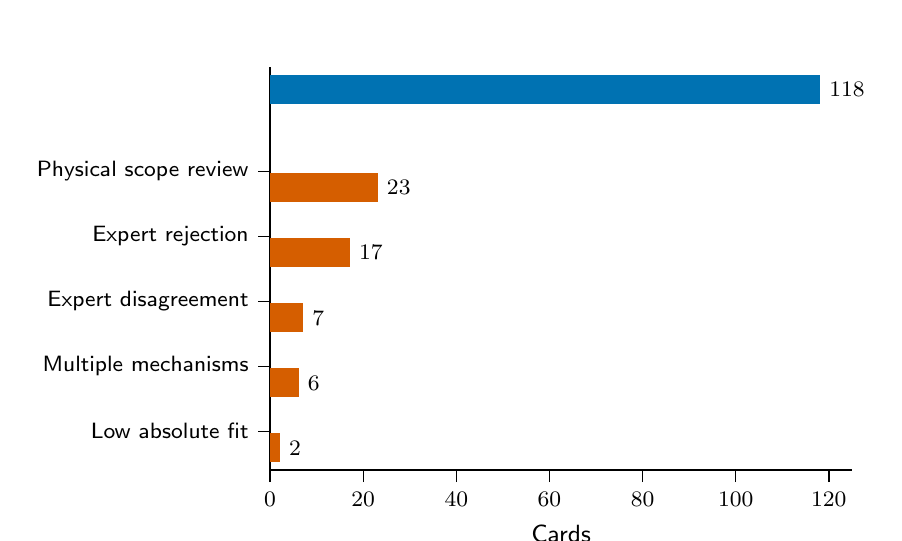
\begin{tikzpicture}
\begin{axis}[
  natureaxis,
  xbar,
  xmin=0,
  xmax=125,
  width=0.74\linewidth,
  height=6.7cm,
  xlabel={Cards},
  symbolic y coords={Low absolute fit,Multiple mechanisms,Expert disagreement,Expert rejection,Physical scope review,Suitability reserve},
  ytick=data,
  bar width=10pt,
  nodes near coords,
  nodes near coords style={font=\sffamily\footnotesize, anchor=west},
  enlarge y limits=0.12,
]
\addplot[fill=naturevermillion, draw=naturevermillion] coordinates {
  (2,Low absolute fit) (6,Multiple mechanisms) (7,Expert disagreement)
  (17,Expert rejection) (23,Physical scope review)
};
\addplot[fill=natureblue, draw=natureblue] coordinates {(118,Suitability reserve)};
\end{axis}
\end{tikzpicture}
\caption{\textbf{Disposition of the 173 Stage 2 holds.} The 55 difficult cases
(vermillion) are force-assigned and marked \code{HOLD}; 118 suitability-reserve
cards (blue) are also force-assigned.}
\label{fig:holds}
\end{figure}

\section{Exploratory analyses}
\label{app:expansion}

\subsection{Candidate L3 families for General and Agentic AI}

The v2.17.1 taxonomy does not add new General or Agentic L3 families. However,
the HOLD reason analysis indicates where future L3 additions are most likely
to improve semantic reliability. The diagnostic rule is conservative: a new L3
is considered only when it explains a recurring HOLD cluster, has a mechanism
that is not already captured by an existing L3 definition, and is likely to
reduce overloaded or ambiguous assignments without fragmenting the taxonomy.
The analysis is therefore a design hypothesis for the next review round, not a
published mapping change.

General AI has the larger improvement opportunity. Of the v2.17.0 HOLD queue,
280 cards are tagged as taxonomy-gap or missing-scope cases, 173 as
Anthropomorphism mechanism ambiguity, and 138 as overloaded-L3 or weak
evidence-fit cases. Keyword and definition review further shows recurring
General-side clusters around governance, transparency, security, dependency,
resources, labor, and power. These clusters are semantically broader than
single L4 labels but narrower than the current L1 or L2 structure, making them
plausible L3 candidates.

\begin{table}[ht]
\centering
\caption{Conservative candidate L3 families for future General AI review.}
\label{tab:general-candidate-l3}
\small
\setlength{\tabcolsep}{4pt}
\begin{tabularx}{\textwidth}{@{}c L{4.4cm} L{2.8cm} Y@{}}
\toprule
Priority & Candidate L3 & Korean label & Expected reliability effect \\
\midrule
1 & Governance and Accountability & \ko{거버넌스·책임성} & Reduces governance and audit taxonomy gaps \\
2 & Transparency and Explainability & \ko{투명성·설명가능성} & Separates documentation, opacity, and explanation risks \\
3 & AI Security & AI \ko{보안} & Separates non-Physical security, attack, and vulnerability risks \\
4 & Dependency and Manipulation & \ko{의존·조작} & Relieves Anthropomorphism over-assignment \\
5 & Resource and Environmental Harm & \ko{자원·환경 영향} & Captures compute, energy, water, and carbon harms \\
6 & Labor and Power & \ko{노동·권력 불균형} & Captures labor, concentration, and inequality mechanisms \\
\bottomrule
\end{tabularx}
\end{table}

The first four General candidates are the strongest. \emph{Governance and
Accountability} directly addresses the largest taxonomy-gap theme, including
audit, regulation, certification, reporting, accountability, and liability
cards that are currently forced into less specific safety families.
\emph{Transparency and Explainability} separates model-card, system-card,
documentation, opacity, and contestability risks from general interaction or
system-safety families. \emph{AI Security} provides a non-Physical home for
prompt injection, poisoning, jailbreak, exfiltration, backdoor, and software
vulnerability risks when the risk mechanism is not specifically embodied.
\emph{Dependency and Manipulation} is expected to improve the overloaded
Anthropomorphism region by moving trust, persuasion, overreliance,
parasocial-bonding, and behavioral-manipulation cards whose operative
mechanism is dependence or influence rather than human-like presentation.

Agentic AI should be treated more conservatively. The prior v2.8.0 expansion
tested four intuitive Agentic families: Goal and Planning, Tool Calling,
Memory, and Oversight and Control. Those families were retired in v2.14.0
because the released L4 counts were sparse and the resulting separation was
not stable enough to justify permanent L3 expansion. The current evidence
therefore does not support recreating those four categories as published L3
families. Two narrower Agentic candidates may still be worth an experimental
ablation because they reflect agent-specific failure modes rather than generic
General AI risks.

\begin{table}[ht]
\centering
\caption{Candidate Agentic AI L3 families for experimental ablation only.}
\label{tab:agentic-candidate-l3}
\small
\setlength{\tabcolsep}{4pt}
\begin{tabularx}{\textwidth}{@{}c L{4.4cm} L{2.8cm} Y@{}}
\toprule
Priority & Candidate L3 & Korean label & Reason for caution \\
\midrule
1 & Tool and Environment Security & \ko{도구·환경 보안} & Agent-specific, but overlaps with General AI Security \\
2 & Traceability and Audit & \ko{추적성·감사} & Agent-specific action provenance, but overlaps with governance \\
\bottomrule
\end{tabularx}
\end{table}

The recommended next experiment is therefore minimal: test the four strongest
General candidates first, then run an ablation with zero, one, or two Agentic
candidates. A candidate should be accepted only if it improves non-HOLD top-1
containment, top-5 containment, median assignment margin, negative-margin
share, and perturbation stability without creating a new sparse or unstable
family. Until that criterion is met, the current v2.17.1 release should remain
unchanged.

\subsection{Counterfactual reliability simulation}

The candidate L3 proposal was tested as a counterfactual simulation rather
than as a release change. The simulation uses the same pinned BGE-M3 card
embeddings as the v2.17.0 audit and evaluates v2.17.1 under three conditions:
the current 50 semantic L3 families, the current taxonomy plus four General AI
candidates, and the current taxonomy plus four General AI candidates and two
Agentic AI candidates. Physical source cards are locked. A card can move to a
candidate family only when its English title or definition matches the
candidate keyword gate and its BGE-M3 similarity to the candidate definition
exceeds its similarity to the current L3 seed by at least 0.012. This is a
conservative automatic gate; it is not a human gold-standard adjudication.

\begin{table}[ht]
\centering
\caption{Counterfactual all-card reliability under candidate L3 expansion.}
\label{tab:l3-expansion-sim-all}
\small
\setlength{\tabcolsep}{4.5pt}
\begin{tabular}{lrrrrrr}
\toprule
Condition & Families & Moved & Top-1 & Top-5 & Neg. margin & Noise 0.05 \\
\midrule
Current v2.17.1 & 50 & 0 & 64.6\% & 92.9\% & 35.4\% & 72.3\% \\
General +4 & 54 & 203 & 63.1\% & 91.9\% & 36.9\% & 71.9\% \\
General +4, Agentic +2 & 56 & 243 & 63.2\% & 91.6\% & 36.8\% & 72.1\% \\
\bottomrule
\end{tabular}
\end{table}

\begin{table}[ht]
\centering
\caption{Counterfactual non-HOLD reliability under candidate L3 expansion.}
\label{tab:l3-expansion-sim-nonhold}
\small
\setlength{\tabcolsep}{4.5pt}
\begin{tabular}{lrrrrrr}
\toprule
Condition & Families & Moved & Top-1 & Top-5 & Neg. margin & Noise 0.05 \\
\midrule
Current v2.17.1 & 50 & 0 & 76.4\% & 95.5\% & 23.6\% & 78.2\% \\
General +4 & 54 & 42 & 75.9\% & 95.9\% & 24.1\% & 77.6\% \\
General +4, Agentic +2 & 56 & 68 & 75.8\% & 95.7\% & 24.2\% & 77.7\% \\
\bottomrule
\end{tabular}
\end{table}

\begin{figure}[ht]
\centering
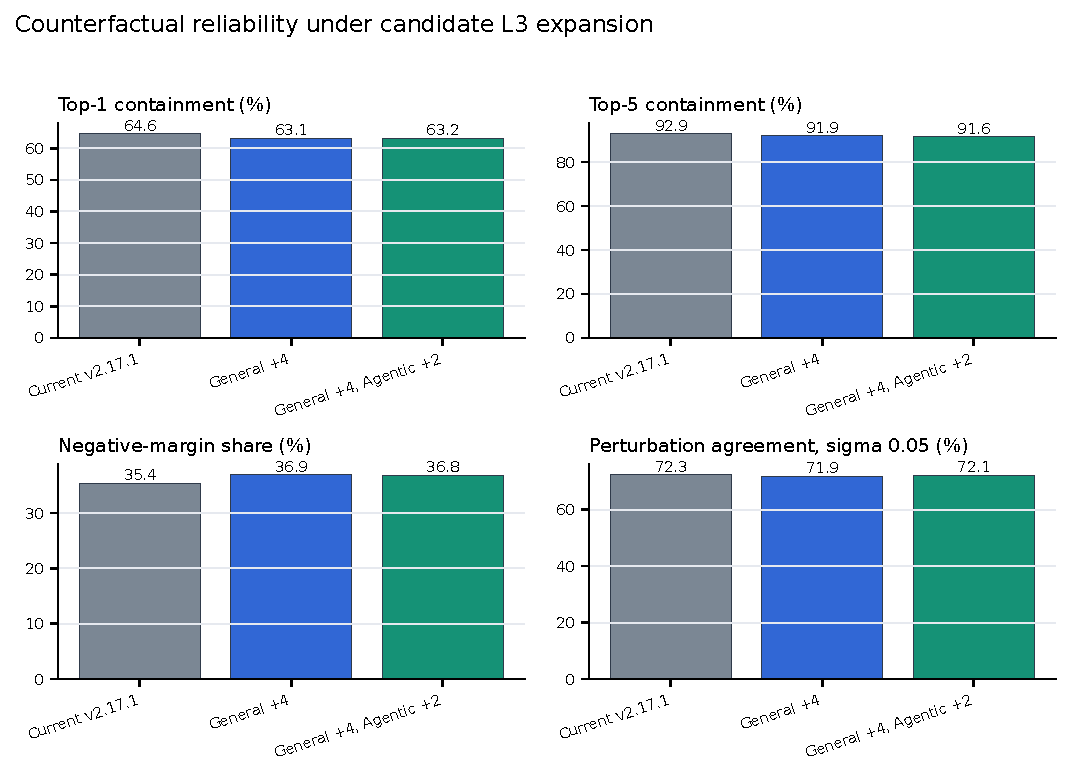
\includegraphics[width=\textwidth]{../validation/v2.17.1/l3_expansion_simulation/candidate_l3_expansion_simulation.pdf}
\caption{\textbf{Counterfactual reliability under candidate L3 expansion.}
Bars compare the current v2.17.1 release with two candidate-expansion
conditions. Higher is better for top-1, top-5, and perturbation agreement;
lower is better for negative-margin share. Candidate expansion creates
plausible movement candidates but does not improve the main reliability
criteria.}
\label{fig:l3-expansion-simulation}
\end{figure}

The simulation does not support immediate L3 expansion. The four General
candidates move 203 cards, including 161 held cards, but all-card top-1
containment falls from 64.6\% to 63.1\%, top-5 containment falls from 92.9\%
to 91.9\%, negative-margin share rises from 35.4\% to 36.9\%, and
$\sigma=0.05$ perturbation agreement falls from 72.3\% to 71.9\%. Adding the
two Agentic candidates moves 243 cards in total but still fails to improve the
main reliability criteria. Non-HOLD results show the same pattern: the
candidate expansions create only marginal top-5 changes while reducing top-1
containment, margin quality, and perturbation stability.

The only metric that improves under the all-card counterfactual is
EM-to-release agreement, rising from 20.6\% to 23.4\% for General +4 and
23.3\% for General +4 plus Agentic +2. This improvement is not sufficient for
release adoption because it is accompanied by weaker top-$k$ containment and
lower stability. The practical conclusion is that the proposed General and
Agentic L3 candidates remain useful review hypotheses, but they should not be
added to the public taxonomy until a human-adjudicated gold set and a stricter
ablation show simultaneous improvement in top-1 containment, top-5 containment,
median margin, negative-margin share, and perturbation stability.

\subsection{Two-dimensional release-state vector space}

Figure~\ref{fig:v2171-domain-vector-space} projects all 1,711 v2.17.1 L4 cards
into a two-dimensional vector space. The input vectors are the pinned BGE-M3
card embeddings used in the v2.17.0 audit; v2.17.1 changes only seven routing
decisions and does not rewrite card text, so the same embedding matrix is
valid for this diagnostic. The projection uses PCA on L2-normalized embeddings.
The first two components explain 5.0\% and 3.8\% of variance, respectively.
The figure should therefore be read as a low-dimensional diagnostic view of
release state, not as proof of discrete taxonomy clusters.

\begin{figure}[ht]
\centering
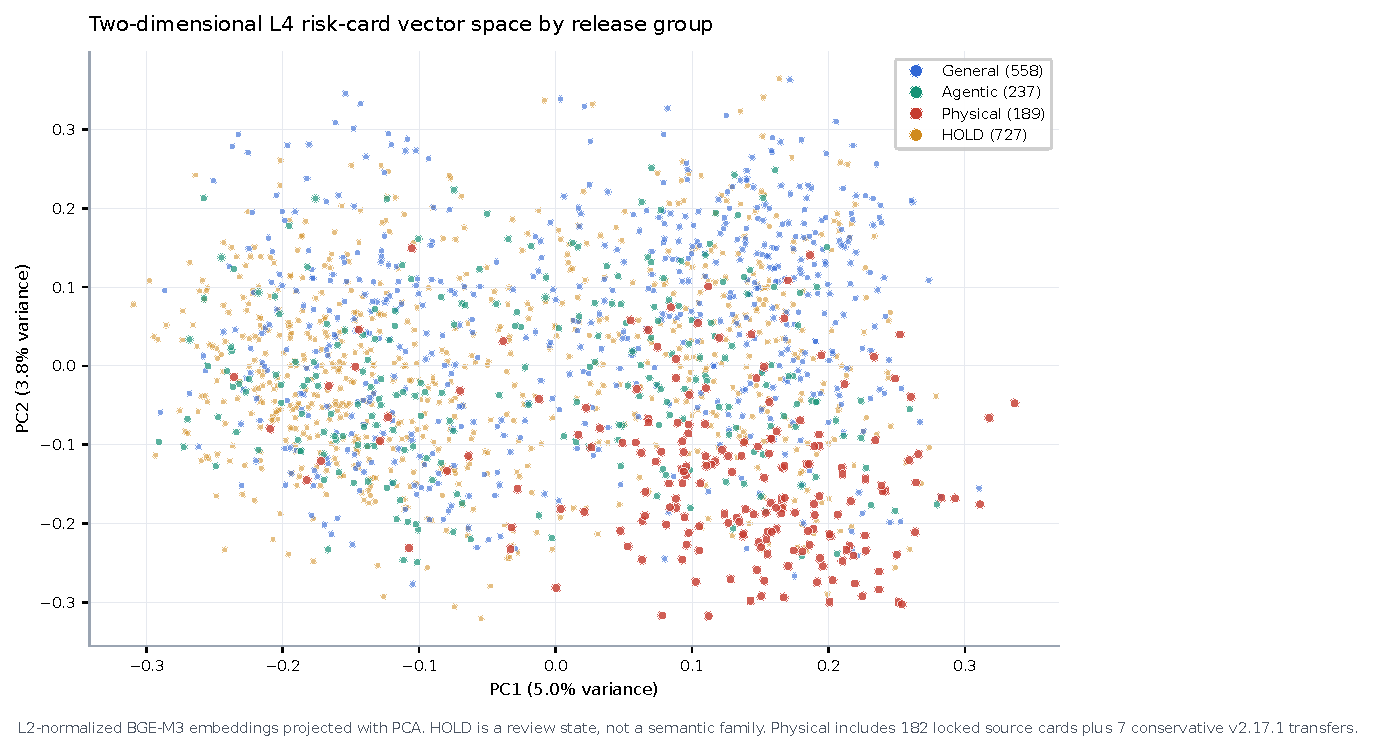
\includegraphics[width=\textwidth]{../validation/v2.17.1/vector_space/domain_hold_vector_space.pdf}
\caption{\textbf{Two-dimensional L4 risk-card vector space by release group.}
Each point is one L4 card. Colors show the public release group after v2.17.1:
General AI, Agentic AI, Physical AI, or HOLD. HOLD is a review state rather
than a semantic family. Physical includes the 182 locked Physical source cards
plus seven conservative v2.17.1 transfers. The overlap between HOLD and the
three semantic domains supports the current interpretation of HOLD as a
cross-cutting adjudication queue rather than a separate risk domain.}
\label{fig:v2171-domain-vector-space}
\end{figure}

\section{Historical reliability results}
\label{app:hist}

\subsection{Full-release results before HOLD separation (v2.12.0--v2.14.0)}

\begin{table}[H]
\centering
\caption{Released-centroid support for the v2.14.0 forced migrations.}
\begin{tabular}{lrrrrr}
\toprule
Subset & Cards & Mean cosine & Median margin & Top-1 & Top-3 \\
\midrule
Migrated v2.14.0 & 39 & 0.746 & -0.005 & 46.2\% & 71.8\% \\
All other cards & 1,672 & 0.769 & 0.013 & 65.1\% & 86.4\% \\
\bottomrule
\end{tabular}
\end{table}

The migrated subset is weaker than the unchanged population: 53.8\% of its
cards have negative assignment margins, and its top-1 containment is only
46.2\%. This result supports the conservative policy decision to retain
\code{HOLD} on every forced migration. It does not invalidate the operational
destinations; it identifies them as priority items for human adjudication.

\subsection{Reliability after excluding HOLD review paths (v2.15.0)}

The second analysis uses the identical encoder, seed, centroid procedure,
5,000 matched-size permutations, and 200 perturbation repeats, but excludes
all 720 HOLD cards before constructing family centroids. It assesses 991
non-HOLD cards across the same 50 semantic L3 families; none of those families
is empty. The two HOLD review nodes are navigation constructs and are not
embedded or treated as risk-family prototypes.

\begin{figure}[H]
\centering
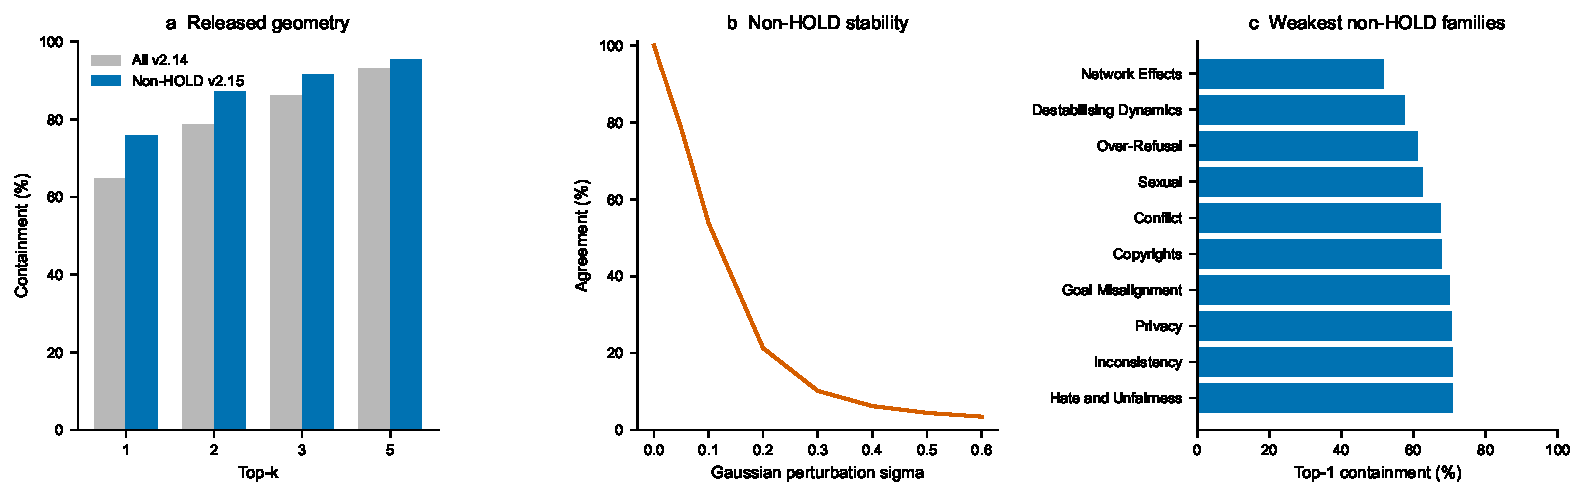
\includegraphics[width=\textwidth]{../validation/v2.15.0/non_hold_reliability/non_hold_reliability.pdf}
\caption{\textbf{Reliability after HOLD separation (v2.15.0).}
(a) Top-$k$ containment for the 991 non-HOLD cards is shown against the full
v2.14.0 population. (b) Perturbation stability is calculated only on non-HOLD
centroids and cards. (c) The ten weakest non-HOLD families identify the next
review priorities.}
\label{fig:nonhold-reliability}
\end{figure}

\begin{table}[H]
\centering
\caption{Reliability with HOLD embedded and after HOLD exclusion.}
\small
\begin{tabular}{lrr}
\toprule
Metric & All v2.14.0 & Non-HOLD v2.15.0 \\
\midrule
Cards assessed & 1,711 & 991 \\
Semantic L3 families & 50 & 50 \\
Mean within-family cosine & 0.768 & 0.779 \\
Median assignment margin & 0.012 & 0.024 \\
Negative-margin share & 35.3\% & 24.2\% \\
Top-1 containment & 64.7\% & 75.8\% \\
Top-2 containment & 78.6\% & 87.3\% \\
Top-3 containment & 86.1\% & 91.5\% \\
Top-5 containment & 93.1\% & 95.4\% \\
EM agreement with released paths & 21.8\% & 31.7\% \\
Agreement at $\sigma=0.01$ & 94.5\% & 95.6\% \\
Agreement at $\sigma=0.05$ & 72.8\% & 78.4\% \\
Permutation p-value & 0.0002 & 0.0002 \\
\bottomrule
\end{tabular}
\end{table}

The conditional non-HOLD subset is more coherent: top-1 containment rises by
11.1 percentage points, the median margin approximately doubles, and the
negative-margin share falls by 11.1 points. EM reaches a fixed point after 13
iterations and agrees with 31.7\% of released paths (adjusted Rand index 0.187;
normalized mutual information 0.501). Observed cohesion is 0.779 versus a
matched-size null mean of 0.742, with zero exceedances and plus-one
$p=0.0002$.

These are not before and after accuracy estimates on the same population. The
later analysis deliberately removes the review-priority cases that were known
to have weaker fit, changes every centroid, and reduces the sample from 1,711
to 991. The improvement therefore validates HOLD as an effective triage
separation signal; it does not prove that every non-HOLD assignment is correct
or that moving a card into HOLD improves its semantic classification.

\subsection{HOLD sensitivity analysis (v2.15.0)}

We next compare the same three diagnostics under two explicit conditions:
\emph{HOLD included}, where all 1,711 v2.14.0 cards remain embedded in their
semantic L3 assignments, and \emph{HOLD excluded}, where the 720 review-path
cards are removed and only the 991 non-HOLD cards are assessed. Both conditions
use BGE-M3 embeddings, seed 20260721, the same 50 semantic L3 families, 5,000
matched-size label permutations, and 200 perturbation repeats. The two HOLD
navigation nodes introduced in v2.15.0 are excluded from centroid construction.

\begin{figure}[H]
\centering
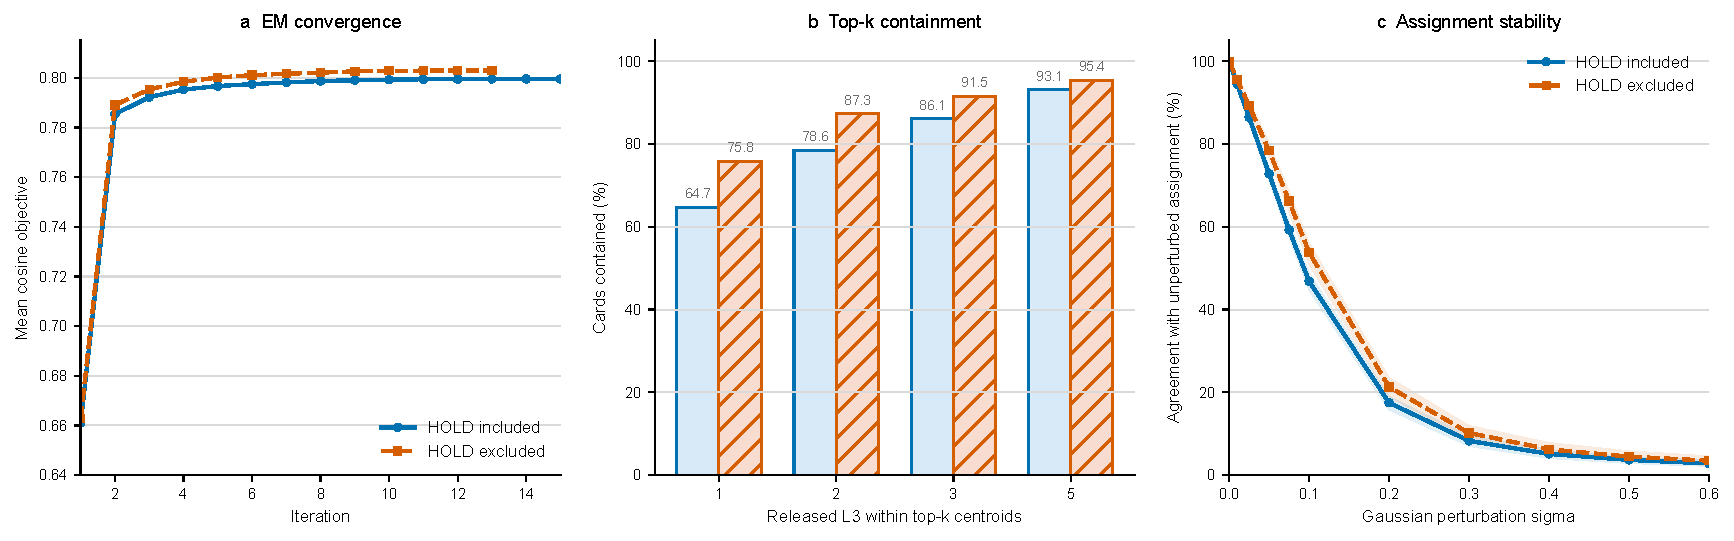
\includegraphics[width=\textwidth]{../validation/v2.15.0/hold_sensitivity/hold_sensitivity_analysis.pdf}
\caption{\textbf{HOLD sensitivity analysis.}
(a) Seed-initialized spherical EM reaches a fixed point after 15 iterations
with HOLD included and after 13 iterations with HOLD excluded. (b) Released-L3
top-$k$ containment improves across $k=1,2,3,5$ after removing HOLD cards.
(c) Assignment stability under Gaussian embedding perturbation is higher on
the non-HOLD subset across the tested noise schedule. Shaded bands indicate
95\% intervals across 200 perturbation repeats.}
\label{fig:hold-sensitivity}
\end{figure}

\begin{table}[H]
\centering
\caption{Sensitivity results with HOLD included and excluded.}
\small
\begin{tabular}{lrr}
\toprule
Diagnostic & HOLD included & HOLD excluded \\
\midrule
Cards assessed & 1,711 & 991 \\
HOLD cards excluded & 0 & 720 \\
EM iterations to fixed point & 15 & 13 \\
Final EM objective & 0.800 & 0.803 \\
EM agreement with released paths & 21.8\% & 31.7\% \\
Top-1 containment of released L3 & 64.7\% & 75.8\% \\
Top-2 containment of released L3 & 78.6\% & 87.3\% \\
Top-3 containment of released L3 & 86.1\% & 91.5\% \\
Top-5 containment of released L3 & 93.1\% & 95.4\% \\
Perturbation agreement, $\sigma=0.01$ & 94.5\% & 95.6\% \\
Perturbation agreement, $\sigma=0.05$ & 72.8\% & 78.4\% \\
\bottomrule
\end{tabular}
\end{table}

The sensitivity result is directionally consistent across the three requested
tests. HOLD exclusion shortens EM convergence by two iterations, raises final
objective from 0.800 to 0.803, increases released-path agreement by 9.9
percentage points, raises top-1 containment by 11.1 points, and raises
$\sigma=0.05$ perturbation agreement by 5.6 points. The correct interpretation
is not that the same cards became more reliable. Rather, the HOLD policy
successfully concentrates low-fit and taxonomically ambiguous cases, leaving a
cleaner subset whose released L3 assignments are more stable under the tested
embedding geometry.

\section{Rounding and reporting policy}
\label{app:rounding}

All counts are reported as integers. Percentages below 1 are rounded at the
third decimal place and displayed to two decimal places; percentages with an
integer component of at least 1 are rounded and displayed to one decimal place.
For example, the L4 registry represents 0.04\% of the integrated AI evidence
count, the AI-risk view represents 2.1\%, final L3 coverage is 100.0\%, and the
decision-required share is 42.1\%. Exact floating-point ratios remain available in the
machine-readable statistics artifact.


\end{appendices}


\vspace{6pt}
\noindent\emph{This document is the restructured journal edition of RAI Risk Taxonomy Technical Report 2.0 at release state v2.17.1.}

\end{document}
